\subsection*{Flujo de caja}
\addcontentsline{toc}{subsection}{Flujo de caja}

El flujo de caja permite realizar un seguimiento al dinero de la empresa, con el fin de evaluar su capacidad para pagar las deudas y cubrir los gastos generados, así como determinar la liquidez del negocio. En la tabla \ref{FlujoCaja} se ilustra con mayor claridad esta información.

\begin{table}[H]
	\centering
	\caption[{Flujo de caja}]{\centering Flujo de caja. \textit{Fuente:} Autores.}
	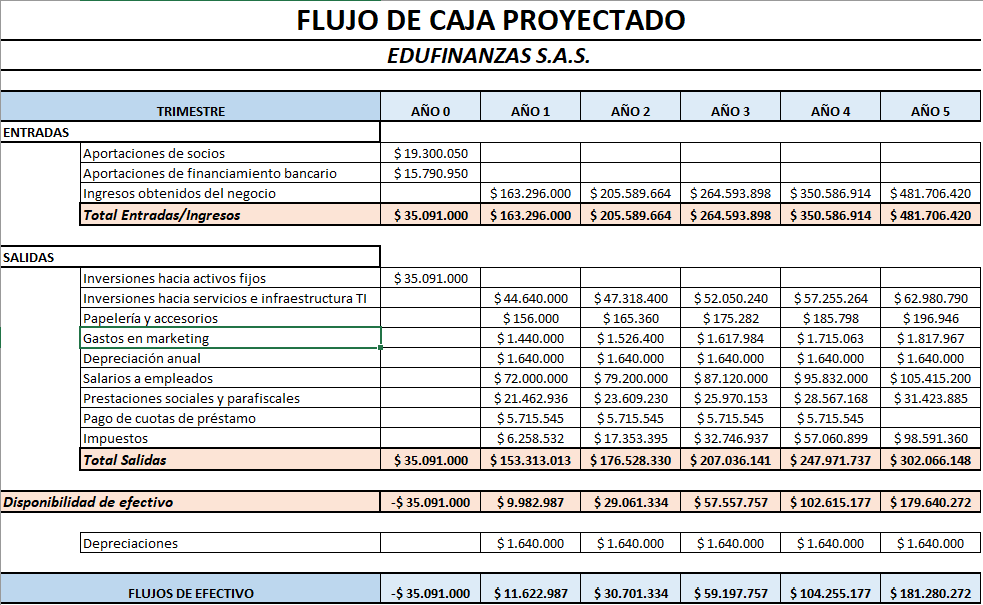
\includegraphics[width=15cm]{Imagenes/FlujoCaja.png}
	\label{FlujoCaja}
\end{table}